%% This file has been modified for the purpose of the Seminar UVIS
%% The original template is available: https://www.overleaf.com/project/5e8c3eb03e447300014bcc5a

%% This is file `sample-uvis.tex',
%% generated with the docstrip utility.
%%
%% The original source files were:
%%
%% samples.dtx  (with options: `sigconf')
%% 
%% IMPORTANT NOTICE:
%% 
%% For the copyright see the source file.
%% 
%% Any modified versions of this file must be renamed
%% with new filenames distinct from sample-sigconf.tex.
%% 
%% For distribution of the original source see the terms
%% for copying and modification in the file samples.dtx.
%% 
%% This generated file may be distributed as long as the
%% original source files, as listed above, are part of the
%% same distribution. (The sources need not necessarily be
%% in the same archive or directory.)
%%
%% The first command in your LaTeX source must be the \documentclass command.
\documentclass[sigconf, nonacm]{acmart}
\usepackage{float}
%%
%% \BibTeX command to typeset BibTeX logo in the docs
\AtBeginDocument{%
  \providecommand\BibTeX{{%
    \normalfont B\kern-0.5em{\scshape i\kern-0.25em b}\kern-0.8em\TeX}}}

%%
%% end of the preamble, start of the body of the document source.
\begin{document}
\graphicspath{ {./images/} }

%%
%% The "title" command has an optional parameter,
%% allowing the author to define a "short title" to be used in page headers.
\title{Improvements of Chatbot-Applications offering Cognitive Behavioural Therapy regarding Security, Privacy and Safety}

%%
%% The "author" command and its associated commands are used to define
%% the authors and their affiliations.
%% Of note is the shared affiliation of the first two authors, and the
%% "authornote" and "authornotemark" commands
%% used to denote shared contribution to the research.
\author{Moritz Pflügner}
\affiliation{\institution{TU Dresden}}
\email{moritz.pfluegner@mailbox.tu-dresden.de}

%%
%% By default, the full list of authors will be used in the page
%% headers. Often, this list is too long, and will overlap
%% other information printed in the page headers. This command allows
%% the author to define a more concise list
%% of authors' names for this purpose.
%\renewcommand{\shortauthors}{J. P. Kumquat}

%%
%% The abstract is a short summary of the work to be presented in the
%% article.
\begin{abstract}
While chatbot-applications in general have become present in areas such as consulting or customer support, they are also implemented
within applications offering Cognitive Behavioural Therapy (CBT). CBT aims to improve a patients mood by changing behavioural patterns and proposing
activities that can help to achive a higher mindfullness.
\\
Two state-of-the art chatbots have been reviewed regarding aspects of Safety, Security and Efficiacy. The review has shown, that they have a positive 
impact on a users mood, take care for sensitive data and can react to critical situations but have also several weaknesses that should be considered. 
\\
As chatbots for mental health belong to Human Computer Interaction (HCI), certain requirements have been reviewed that an application should meet. This review has shown
that users trust high-quality chatbots with sophisticated responses more while having less privacy concerns at the same time. Furthermore, the deletion and 
inappropriate use of data are the two aspects, users worry the most about. 
\\
Based on the review of the existing chatbots and the requirements, three options have been proposed who aim to meet them.
The Knowledge and Data Dashboard, that constantly allow access to saved data and offers options like data deletion, 
the Chatbot Setup Phase that try to personalize the application as much as possible to improve the general user experience and 
a Safety Certificate, that ensures the appropriate handling of critical situations.   
\end{abstract}

%%
%% Keywords. The author(s) should pick words that accurately describe
%% the work being presented. Separate the keywords with commas.
\keywords{}

%%
%% This command processes the author and affiliation and title
%% information and builds the first part of the formatted document.
\maketitle

\section{Introduction}
During the last two decades the internet has become a major part in the life
of people throughout the society. The ubiquity has led to the desire for 
location-independent usage. As a consequence the amount of
smartphone users is increasing every year.\footnote{https://www.statista.com/statistics/330695/number-of-smartphone-users-worldwide/, last access: 13.05.2021}
With constant access to the biggest collection of knowledge in the world,
more and more individuals tend to use it as a first source of information when
symptoms of illness arise\cite{Wyatt2015}. 
In terms of mental health, the internet provides a numerous amount of \emph{cognitive behavioural therapy} (CBT) offers such as guides
or apps. 
\\\\
In contrast to a complex psychoanalysis with the guidance of a therapist or doctor trying to look into the past,
CBT focuses more on the way an individual deals with its present thoughts and beliefs. The treatment has the aim to
change behavioural patterns in a way that they positively influence emotions and cognition. CBT is based on this connection
between the way how we interpret the daily life, how we behave due to it and how we 
feel in the end which is shown in Figure \ref{fig:cbt_circle}. By changing one of the three aspects,
the others are changed as well automatically. Some popular methods are keeping a \emph{Gratitude Journal} or exercises to calm the body.\cite{Spangler2002}
\\
\emph{Gratitude Journaling} works by writing down moments, situations or facts the writer is grateful for. It can lead to a more positive mindset and higher mindfulness. 
\begin{figure}[h]
  \centering
  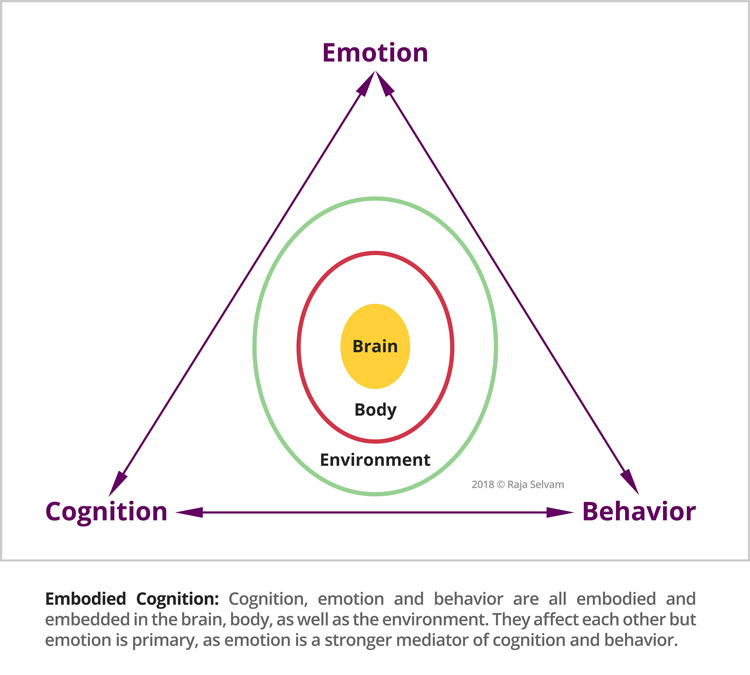
\includegraphics[width=\linewidth]{cbt_picture}
  \caption[cbt_circle]{The relationships among cognition, emotion, behavior. Graphic by Raja Selvam, 2018\footnotemark}
  \Description{The relationships among cognition, emotion, behavior.}
  \label{fig:cbt_circle}
\end{figure}
\footnotetext{https://integralsomaticpsychology.com/wp-content/uploads/2018/02/ISP-Embodied-Cognition-Diagram-Raja-Selvam-750.jpg, last access: 30.04.2021}
\\
With the help of apps, users can get hints and instructions to conduct self-help. It is possible
to get first support without the need to consult a therapist or doctor. Often, this a big and 
difficult step for many people due to the fear of getting stigmatized\cite{Rossler2016}.
While CBT applications have the potential to reduce the barrier to seek help, the rate of completion
is relatively low. Donkin et. al \cite{Donkin} found a median minimal completion rate of 56\% during a randomized controlled trial. 
One possible reason for this lack of adherence is the missing human interaction of internet-based CBT\cite{Ly2017}.
The usage of chatbots are considered as a possible solution for this problem. While they are providing CBT on the same level 
as non-chatbot based approaches, they can deliver an artificial human interaction that is supposed to increase the
therapy adherence which can be seen as an important aspect of a successful therapy. 
\\\\
The paper starts with a review of the conducted research and analyses weaknesses and strengths as well as risks and chances. 
Subsequently, it will analyse some general requirements a chatbot used for CBT should met.
What are aspects that need improvement during further development approaches and what methods and measures might be suitable to achive that? 
Considering the state of the art and the general requirements, the paper tries to answer this question regarding safety aspects, efficiacy and privacy.
It finally discusses the outcomes and points out limits of chatbot based CBT.



\section{Strenghts and weaknesses of existing chatbots}
This far, there are a couple of chatbots available. This paper will mainly focus on the \emph{Woebot} Chatbot and \emph{Wysa} for several reasons.
On the one hand, they have been developed in a research oriented context. 
The examples are available in english language and free to use.\footnote{https://woebothealth.com/about-us/, last access: 01.05.2021}\textsuperscript{,}\footnote{https://www.wysa.io/faq, last access: 01.05.2021}
\\
Additionally, the developers provide numerous information on their website
like experience reports or technical aspects.
On the other hand, a lot of studies have already been conducted mainly focusing on the efficiacy of the chatbot based CBT. 
They revealed some weaknesses of those chatbots, some chances and also risks concerning Efficiacy, Privacy and Safety.

\subsection{\emph{Woebot}}
The \emph{Woebot} chatbot is a product of the company \emph{WoebotHealth} which has its headquarter in California. It is the reusult of a resarch 
project at the university of Stanford in 2017 and has raised 8.000.000 dollars of funds.
\emph{Woebot} is available as a standalone app in \emph{Apple}'s App Store and in \emph{Google Play} store where it reached more than 100.000 downloads\footnote{https://play.google.com/store/apps/details?id=com.woebot\&hl=de\&gl=US, last access: 03.05.2021} and as 
a \emph{Facebook} chatbot. It is based on natural language processing and offers free-text inputs as well as predefined answers.
In general, it gives hints how to change the thinking and guides the user through techniques such as \emph{Gratitude Journaling}. 
Based on the answers it creates a graph monitoring mood changes during the week.
\emph{Woebot} aims to reach patients and clinicians. While users that are currently not in therapy have the opportunity to use it,
it can also improve and support ongoing therapies clinicians are conducting.
Currently, the usage of \emph{Woebot} is completely free of charge. Nevertheless, \emph{Woebot} Health announces on its website, that they are moving forward
to develop a more sustainable business model which could lead to costs for the users.\footnote{https://woebothealth.com/about-us/, last access: 01.05.2021}\textsuperscript{,}\footnote{https://emerj.com/ai-application-comparisons/chatbots-mental-health-therapy-comparing-5-current-apps-use-cases/, last access: 03.05.2021}
\\\\
A randomized controlled trial with college students by Fitzpatrick et. al \cite{Fitzpatrick2017} has shown that the usage of \emph{Woebot} significantly reduces
symptoms of depression compared to a control group that only got informed about depression via an e-book. Regarding anxiety symptoms, no difference between
both groups has been found but both showed a reduction of it. The results have been examined with the help of the PHQ-9 questionnaire for depression symptoms and the GAD-7 questionnaire for anxiety. Furthermore, the study has revealed that 85\% of persons in the chatbot group used 
it daily or almost daily which can be considered as high in comparison to conventional CBT applications\cite{Ludden2015}.
After the period of two weeks the users have been asked to assess their experience with \emph{Woebot}. One the one hand, the majority appreciated the daily check-ins of the bot 
which motivated them to continue the therapy. On the other hand, many of them noted that the conversations did not feel natural which can be considered as a limit of chatbots
and natural language processing in general.\cite{Fitzpatrick2017}
\\\\
The privacy policy of \emph{Woebot} gives some useful information about the way the chatbot deals with user inputs. 
During the registration process the user will be asked for an e-mail adress and a password. It is possible to skip
this step. Hence, no account will be created and the user wont be able to use the application across devices. 
Additionally, neither access to stored data nor backup functionalities are possible. If a user creates an account, \emph{WoebotHealth} stores
data concerning account information (personal information), technical aspects (platform, operating system), financial information if 
services are purchased, hardware information and analytical data. On the other hand, the company also stores the conversation data in order
to improve the services. \emph{WoebotHealth} also obtains data from other sources. If the service is used trough third-party applications, 
it collects data that has been made public by the user. Examples for third-party applications are social networks or app stores. 
The company does not share information with third parties, but it doesn't have direct control of data that is stored if the chatbot
is used through them like \emph{Facebook's} messenger. The access and deletion of it then depends on \emph{Facebook's} privacy policy.\footnote{https://woebothealth.com/privacy-webview/, last access: 04.05.2021}
\\\\
As chatbots for CBT interact with people who might have serious mental problems, safety and the recognition of emergency situations are important
aspects. If a user starts a conversation with \emph{Woebot}, the bot early advises that it is not a human being. It notes that it has limited capabilities and that it might 
be better for some individuals to see a real therapist. In order to discourage over-reliance, \emph{Woebot} tries to end conversations after a certain amount of time and proposes many non-digital activities in the real world.
Those proposals of non-technology-based activites are part of evidence-based recommendations for mental health app development\cite{Bakker2016}.
Considering emergency situations, \emph{Woebot} is able to recognize user inputs e.g 'SOS' or 'suicide' as such. It reacts with a list of helplines
which can provide further support.\cite{Kretzschmar2019}

\subsection{\emph{Wysa}}
The \emph{Wysa} Chatbot, developed by \emph{Touchkin}, has certain commonalities but also major differences in comparison to \emph{Woebot}. It is also a mobile chatbot app using a text-based interface with the possibility of entering 
free-text input or predefined answers. The biggest difference is the option of having contact to 
a human therapist while using \emph{Wysa}. It is a chargeable feature which costs 29.99\$ per month. The usage of the chatbot without it is free of charge. It is available
in \emph{Apple}'s app store and \emph{Google Play} store where it has been downloaded more than 1.000.000 times\footnote{https://play.google.com/store/apps/details?id=bot.touchkin, last access: 05.05.2021}. 
The company is located in Bangalore and has been found in collaboration with a research team from the universities of Cambridge and Columbia.
While also offering CBT like \emph{Woebot}, \emph{Wysa} also offers guided meditation, breathing and yoga. Additionally, it conducts \emph{Dialectial Behaviour Therapy} (DBT).\textsuperscript{6} 
\\
DBT is a special type of CBT and focuses more on the way a patient deals with emotions and is suitable for patients with self-destructive behaviours. Common techniques are practicing mindfullness or 
improving relationships to other individuals.\footnote{https://www.skylandtrail.org/4-differences-between-cbt-and-dbt-and-how-to-tell-which-is-right-for-you/, last access: 06.05.2021} 
\\\\
Inkster et. al \cite{Inkster} have shown that patients with a more frequent use of \emph{Wysa} have a significantly higher improvment of their mood than users
with a less frequent usage. Their participants were human-beings around the globe who have been asked to install the Wysa app. One part of them used the app less often than the other one. O In general, both groups showed an improvement. 74\% of the study participants provided an in-app feedback. Most of them preferred the pre-defined answers rather than free-text.
While the app was generally considered as helpful and encouraging, the participants proposed improvements included wanting to avoid repetitions or a better understanding of user inputs.
\\\\
The way \emph{Wysa} stores user data deviates from \emph{Woebot}'s. Though \emph{Wysa} does not require a registration, it links all the collected data to a vendor-specific user id provided by \emph{Google Play} or App store. This approach leads to a pseudonymised data storage.
If a user accidentally submits personal information during a conversation, it will be redacted by algorithms scanning the stored data regularly. In addition to conversational data, \emph{Wysa} stores anonymized technical data (platform, operating system), 
financial data if an individual subscribes to paid offers and analytical data in order to improve their services. 
It is important to mention, that the chatbot can not be used through third party applications like \emph{Facebook's} messenger. Hence a user can use the application more independently of privacy policies of other companies. Altough it is not completely excluded as \emph{Wysa} allows to speak with the chatbot 
via \emph{Apple}'s Siri or \emph{Google's} voice assistant.\footnote{https://legal.wysa.io/privacy-policy, last access: 08.05.2021}
\\
The chatbot understands words such as 'privacy' and can provide links and information about it during a conversation as well.\cite{Kretzschmar2019}
\\\\
Considering privacy aspects, \emph{Wysa} is quite common to \emph{Woebot}. It also informs the user during the conversation, that it is only a robot. If an individual is willing to pay the fee, the contact to a human therapist is a safe way when it has mental issues that are 
more serious. But as this service is not free of charge, it can not be seen as a general safety aspect. The \emph{Wysa} chatbot tries to deal with emergency situations the same way as \emph{Woebot} does. It notices user inputs like 'SOS' and provides helplines for further support.\cite{Kretzschmar2019}
\section{General requirements}
This chapter will define requirements a chatbot should meet regarding privacy, efficiacy and safety. Those three aspects have already been examined by Kretzschmar et.al \cite{Kretzschmar2019}, but only from the perspection of young adults as a result of a group discussion.
\\
Due to the fact that the usage of a mental health chatbot belongs to Human Computer Interaction (HCI), the following requirements will be based on its principles and research conducted in the field.

\subsection{Privacy}
Alongside the development of the internet of things, technologies and the amount of data are continously increasing\cite{Reinsel2018}.
As a consequence of it, governments around the globe define rules in order to protect the individual from exploitation and to ensure that users have access and control over personal data stored by service providers.
An example for it is the General Data Protection Regulation by the European Union. Considering chatbots for mental health, privacy is an important aspect. Sharing sensitive and personal information is part of the concept of CBT and hence necessary for a successful chatbot usage. Therefore the user should constantly feel secure its data is being stored properly. 
\begin{figure}[h]
  \centering
  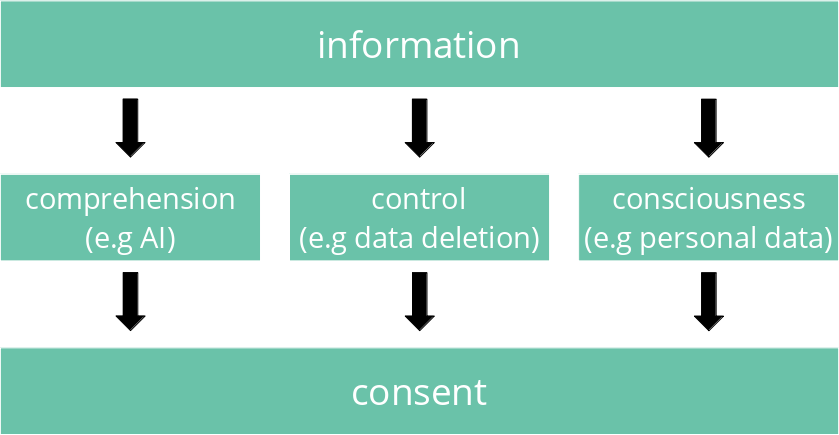
\includegraphics[width=\linewidth]{privacy_base}
  \caption{The connection between information, comprehension, control, consciousness and consent, Graphic by Moritz Pflügner, 2021}
  \Description{The connection between information, comprehension, control, consciousness and consent}
  \label{fig:privacy_base}
\end{figure}
\\
Firstly, it is necessary to define what privacy principles are concerning HCI. In this paper, the results of Patrick and Kenny \cite{Patrick2003} are used, who specifically derived privacy aspects by using the general EU legislation as basis.
They assessed, which principle of the EU legislation might have an implication to HCI and how methods and techniques of HCI could comply it. The result is a grouping of the principles into four categories: \emph{Comprehension} means that an individual understands what is happening to its data. \emph{Consciousness} aims to ensure
awareness of the individual and that it is informed about data processing constantly. \emph{Control} contains principles to have access to stored data and to be empowered to delete it and requirements of the \emph{consent} category make sure that the user always has to give its approval about processing of personal data.
\\
As chatbots are only a subset of HCI and the categories and principles above are held general, it is important to concretise them regarding mental health chatbots.
\\
Saglam et. al \cite{Shamim2021} conducted an empirical study where on the one hand, the participants have been asked to answer questions about their trust towards a chatbot and 
on the other hand, what aspects would lead to worries. Regarding the first question, they found that users are most worried about how to delete personal information. Another aspect was the concern if the data would be used in an inappropriate way. 
For the second question, the study has revealed that users prefer chatbots with good technical quality like grammatically correct answers rather than those with social aspects such as seeing an avatar while chatting.
\\
Chatbots with a better response quality can be seen as more human-like. Ischen et. al \cite{Ischen} revealed in another study, that human-like chatbots lead to less privacy concerns.
\\
The conclusion of both results is that users prefer human-like chatbots while having less privacy concerns at the same time during the conversations. Companies could easily exploit this fact. In order not to be accused of it, they should focus on privacy especially when they are programming chatbots on a professional level.  
Another aspect that has not been considered yet is the distinction between data and information.
\\
An interview with employees about their attitude towards a workplace robot conducted by Lee et. al \cite{Lee2011} showed that most participants did not make a distinction between the knowledge of the robot and the data it collects.
The comparison between a physical robot and a chatbot is limited, but the distinguishing betwen data and information can be applied to chatbots as well. It is necessary for chatbot users to know, what inferences it can make based on the conversational text inputs they are providing. The underlying artifical intelligence a chatbot has should be transparently explained 
to the user in order to raise awareness for problems that can come with intelligent algorithms such as false positive classifications.
\\
In order to summarize the privacy requirements of a chatbot for mental health it can be said, that information is the most important one. Firstly, it leads to a conscious usage of the application which is essential to protect personal data. Secondly, information is necessary in order to know how data can get deleted or accessed. It finally helps to understand the system and 
its algorithms better. Only with all of these aspects given, the individual is able to give its consent on a proper basis as shown in Figure \ref{fig:privacy_base}. 
\subsection{Efficiacy}
Mental health applications always aim to increase the general subjective well-being of a person. Therefore, it can be seen as a measure of an application's efficiacy.
\\    
Ludden et.al \cite{Ludden2015} proposed two different routes that can lead to a better well-being that are shown in Figure \ref{fig:routes}. They introduced the PERMA abbrevation which stands for positive emotions, engagement, positive relationships, meaning and accomplishment. All of these aspects can lead to a higher adherence and hence to a better well-being.
\\
\begin{figure}[h]
  \centering
  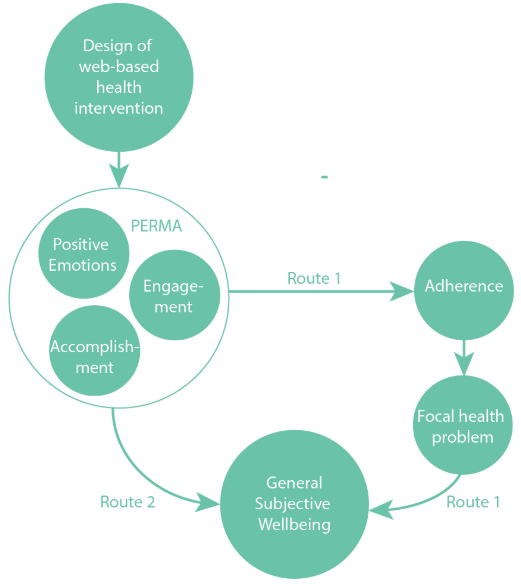
\includegraphics[width=\linewidth]{routes}
  \caption{Schematic representation of how the design of a Web-based intervention can influence general subjective well-being following two different routes. Route 1 indicates the impact of design on adherence and thus on the focal health problem. Route 2 indicates how overall well-being is stimulated by elements of PERMA. Graphic by Ludden et.al \cite{Ludden2015}, 2015}
  \Description{Routes to general subjective wellbeing.}
  \label{fig:routes}
\end{figure}
\\
While the efficacy studies of both chatbots reviewed in chapter two showed a reduction of mental illness symptoms, the adherence of e-therapy applications in general is relatively low.
\\
Donkin et. al \cite{Donkina} found a minimal completion rate of 56\% concerning online-therapy applications. Furthermore they revealed that the adherence correlates with the treatment outcomes.
\\This can be considered as a further prove for Route 1 in Figure \ref{fig:routes}.  
A couple of general design approaches promising an increase of therapy adherence are now being discussed.
\\
Ludden et. al \cite{Ludden2015} present personalization as one approach. Considering the PERMA abbrevation, personalization encourage the engagement of a user as the application has a higher personal relevance. If it is used by multiple groups of people, it should be adaptable to them in order to improve the experience.
Secondly, they discuss an approach that prevents too much ambient information. They point out, that due to the daily information overload in the internet, users might not feel the desire to use the
application online. Additionally it is possible, that individuals have made bad experiences with too much information that concerns the application but is irrelevant for the acutal usage. 
Ludden et. al propose that users should not be overloaded with unneccessary information. According to them, this would lead to a more pleasureable experience (P in PERMA) and a better feeling of accomplishment (A in PERMA).
Finally, they are recommending the use of metaphors for applications concerning mental health. Challenges, goals and experiences should be shaped into words and visualizations in a way to create a meaningful (M in Perma) and engaging (E in Perma) frame.
They note that the way how human beings think about abstract things like challenges or achivements is methaphorical by nature and experienced every day. Metaphors supporting mental health applications can strengthen those experiences.
\\
An application which is personalized as well as focusing only on necessary information and using a sophisticated way to frame challenges and goals resembles a therapy with a human therapist.
\\
According to Ischen et.al \cite{Ischen}, services with a higher perception in anthropomorphism lead to a better adherence.
\\
This result corresponds to the results of Ludden et.al and hence supports the recommendation to implement the PERMA principles in applications for mental health like chatbots. 
\\
\subsection{Safety}
The safety aspects of mental health chatbots are very specific due to the target group and the conversational aspect. Hence, only aspects that are directly related to them will be discussed.
As they reach persons with symptoms of mental illnesses by nature, safety aspects should not be neglected. 
\\
Kretzschmar et. al \cite{Kretzschmar2019} defined four requirements that are essential. Firstly, it is considered as crucial that users get informed about the fact that they are talking to a robot. This makes sure that they are aware of limitations and that the conversation can not replace a real life therapy.
Secondly, they argue that the system should prevent over reliance so that users always keep in mind that the application is only a tool. 
Due to the limitation of a chatbot based conversation, they thirdly recommend that chatbots should additionally encourage seeking human support.
Kretzschmar et. al finally value the recognition of emergency situations.
\\
This last aspect has also been recommended by Grové \cite{Grove2021} who co-developed a chatbot with and for young people. She points out that the identification of critical words is necessary for a chatbot that deals with mental health.
Furthermore she recommends the generation of appropriate answers to those critical words in order to prevent rash reactions.
As a second aspect she notes that the applications should have a sufficient listening phase prior to quick responses that might not be suitable to the situation. 


\section{Methods for Improvements}
After reviewing two chatbots for CBT and analysing requirements for HCI applications in general, some specific development recommendations are now being derivated. 
\subsection{Knowledge and Data Dashboard}
In order to respect the privacy and take user concerns serious, chatbot applications should only exist as a standlone app without the possibility to use it through a third party application such as \emph{Facebook}'s messenger. The dependence of another company's privacy policy excludes control which is a crucial aspect within the 
work of Patrick and Kenny\cite{Patrick2003}. Third party applications can still be used as marketing platforms.
\\
Furthermore, chatbot developers could implement a knowledge and data dashboard. A standalone app could have an extra view which is meant to access and control the data a chatbot has collected.
This approach could have two major advantages. On the one hand, the chatbot user would always be able to get an insight into data that has been gathered. Additionally, those data could be enriched with the chat snippet or user input that has been the source of it. 
This mapping of data and information would probably lead to a better understanding of both concepts in general and how the chatbot infers knowledge in particular. It would contribute to the result of Lee et. al \cite{Lee2011} who noted that users do not distinguish between data and information.
In order to improve transparency basic information about the used algorithm could be provided for users with specific interest or a technical background as well.
\\
On the other hand, it could lead to a more transparent privacy policy and less complex administration processes for the developing companies. Several privacy legislations force companies to give customers access to their stored data. Usually, users have to write an e-mail that needs to be processed by the company. It could save this effort by
implementing the data and knowledge dashboard giving users access to their data constantly.
\\
Moreover, the dashboard could have the option to delete the data. As Saglam et. al \cite{Shamim2021} have shown, chatbot users are worried about how they can delete personal information. Having the possibility to do it directly in the app could lead to a higher trust of the users and again to less complex administration processes for the company
as they would not need to process deletion requests anymore.
\\
The implementation of a knowledge and data dashboard is one possible solution to sharpen the privacy focus. It is also conceivable to integrate the functionalities of the dashboard directly into the chat.
A user input such as 'What do you know about me?' or 'What data have you collected so far?' could lead to an overview of the data in the same manner a dashboard would provide it.
Requests like 'Delete the data!' could then start the wiping process. 
Considering the distinguishing between data and information, questions like 'How did you come to the conclusion that I like rain?' could result in a detailed explaination how the chatbot infered this knowledge.
\\
To summarize the idea of a knowledge and data dashboard it can be said that it has the potential to improve the trust of the users while simplyfing adminstration processes of the company at the same time. 
It would improve the comprehension of the system, giving a human-being control over the data collected by the chatbot and would finally lead to a higher consciousness what kind of personal data is stored.
\subsection{Chatbot Setup Phase}
Chapter 3.2 has presented the PERMA abbrevation by Ludden et. al \cite{Ludden2015} which stands for certain aspects which could improve the efficiacy of a chatbot. A specific development approach which respects PERMA could be the implementation of a quick setup phase prior to the actual chatbot usage.
During it, the chatbot could ask questions that aim to reach a better personalization of the application. Following points could be considered and asked. The Chatbot Setup Phase could be seen as an equivalent to a preliminary talk with a human therapist.
\\
\begin{itemize}
\item\textbf{Age}\\ 
Nowadays, the internet is used by all generations\footnote{http://www.ipsos-mori-generations.com/Internet-and-Technology-Use.html, last access: 22.05.2021}
Therefore, personalization concerning the user age might be useful. Differences between a personalization for younger people and users who are older could be a different set of questions that are asked in order to examine the current mood.
Younger people probably feel more noticed if the chatbot asks about the school routine while questions regarding the workplace should address people of older generations.
\\
\item\textbf{Name}\\
Addressing someone with its name is a quite common personalization approach in current applications and already implemented for Wysa and Woebot. It should be also considered for future developments.
\\
\item\textbf{Design Preferences}\\
While the consideration of the age can directly influence the questions asked during the conversation, aspects such as the design do not influence the dialog but could help to improve the acceptance of the application if the appearance adapts to user preferences. 
\\
\item\textbf{Feedback}\\
A common approach of chatbot based CBT is the recommendation of certain methods. The chatbot could ask after the accomplishment of a method if the individual liked it or not which would be useful knowledge for further method recommendations. It does not fit in the Chatbot Setup Phase but could
be asked during the daily dialogs.
\end{itemize} 
Additionally, too much ambient information should be avoided and the main functionality should be focused. An argument against it could be the funding of the app. The reviewed examples \emph{Woebot} and \emph{Wysa} do not advertise within the application but it is a conceivable approach which leads 
to a trade-off that has to be made. It could be part of future research how advertisements are seen as disturbing ambient information and if they negatively influence the outcomes. 
\\
\subsection{Safety certificate}
As Grové \cite{Grove2021} points out, chabots for mental health should notice and react to critical situations in a sophisticated way due to the vulnerable target group. While the reviewed chatbots meet the requirements, Kretzschmar et. al \cite{Kretzschmar2019} defined,
no information is provided about how they infer if a situation might be critical. In order to improve the general transparency and to ease the assessment if the application can be used in a therapeutical manner, the developing companies could publish on their website either how the machine learning model of their applications infers 
a critical situations or what keywords lead to it in terms of natural language processing.\\
Another conceivable aspect which would make sense if the supply and demand for mental health chatbots continues to grow is the awarding of a safety certificate issued by an independent company or institute. This certificate could include certain aspects which therapists and doctors consider as crucial for the safety of a chatbot.\\ 
Clinicians could assess easily with the help of this certificate if the application is suitable for a therapeutical usage.\\
Furthermore the certificate could be expanded for Privacy Issues and Efficiacy as well which would turn the certificate into a general quality feature for mental health chatbots.
\section{Conclusion}
Nowadays, the amount of people who use the internet as first source of information has increased \cite{Wyatt2015} while it offers many applications for CBT such as chatbots. 
\\
Current and popular examples like \emph{Wysa} or \emph{Woebot} are available as a standalone app or through third party applications. Studies have shown that their CBT is efficiant \cite{Fitzpatrick2017,Inkster}, but in order to improve it and to tackle problems such as missing trust in a chatbot, further improvements could be implemented like personalization 
or the provision of more transparency. To achive that, a chatbot setup phase has been propsed in which specific questions could be asked concerning preferences and personal aspects of the user. It could be considered as the preliminary talk prior to the therapy a human therapist conducts.
The chatbot setup phase would lead to an implementation of the PERMA aspects, that Ludden et. al \cite{Ludden2015} propose and which have been presented in chapter 3.2. Those aspects are promising to increase the general well-being of a user and hence the efficacy of the chabot application.
\\
The developing companies of both reviewed chatbots transparently explain what data is stored for what purpose.\\
Nevertheless, the review of general requirements for HCI applications has shown, that more information about data collection should be provided and how it is possible for the user to delete it.\cite{Shamim2021}
\\
Furthermore, users are not distinguishing between data and information.\cite{Lee2011}
In order to tackle those aspects, a knowledge and data dashboard is proposed that constantly provides information about the data the chatbot has collected and what it did derive from it.
The main advantages are the constant access to personal and sensitive data on the one hand. On the other hand, the provisioning of it could simplify administration processes such as deletion requests as they are done automatically.
\\
Considering Safety aspects, the reviewed chatbots already meet the requirements Kretzschmar et. al \cite{Kretzschmar2019} propose. Both of them explain that they are just robots and engage the user to do non-digital activities to prevent over-reliance.
The only option to figure out if the user notifies and react to critical situations is trial and error. In order to improve the transparently, a certificate is suggested, that could consider certain aspects doctors or therapists consider as crucial.
This certificate could be expaneded to other aspects which could result in a quality feature for mental health chatbots.



%%
%% The next two lines define the bibliography style to be used, and
%% the bibliography file.
\bibliographystyle{unsrt}
\bibliography{library}

%%
%% If your work has an appendix, this is the place to put it.
\appendix

\end{document}
\endinput
%%
%% End of file `sample-uvis.tex'.
